\section{Introduction}
Correctly determining if a person has inflammation in the ear can be difficult. Using image analysis and machine learning on a good data set, the expectation is that it is possible to reduce the amount of antibiotics used on ear inflammations, as diagnosing correctly would be much easier.\\
Creating this data set requires sorting away pictures of poor quality. The images are taken with an otoscope, which is a device that is placed in the ear canal from the outer ear, and makes it possible to see the eardrum. Some possible complications with the otoscopy images are:

\begin{figure}[H]
    \centering
    \begin{subfigure}[t]{0.32\textwidth}
        \centering
        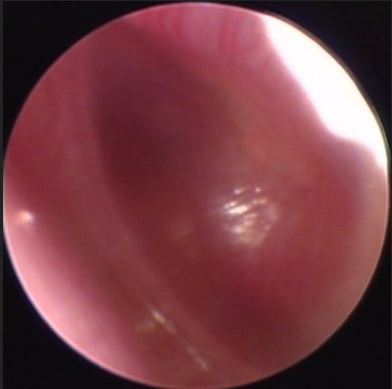
\includegraphics[width=2.5cm]{Figures/Intro/ear5.png}
        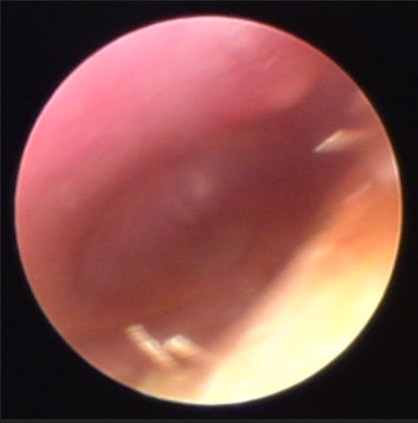
\includegraphics[width=2.5cm]{Figures/Intro/ear6.png}
        \caption{The image is out of focus}
        \label{fig:intro_blur}
    \end{subfigure}
    \begin{subfigure}[t]{0.32\textwidth}
        \centering
        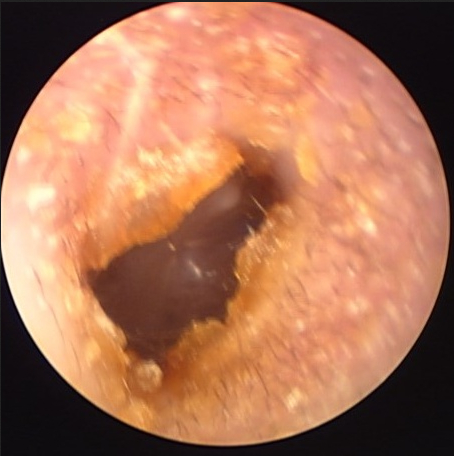
\includegraphics[width=2.5cm]{Figures/Intro/ear3.png}
        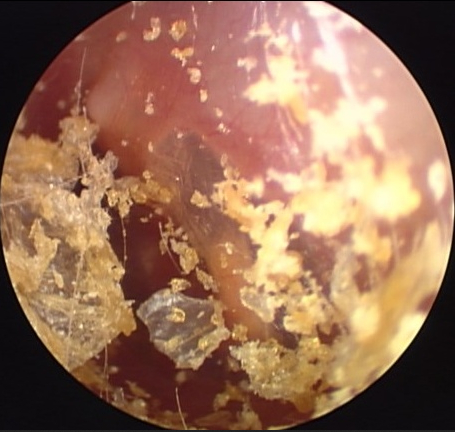
\includegraphics[width=2.5cm]{Figures/Intro/ear4.png}
        \caption{There is too much ear wax to see the membrane}
        \label{fig:intro_wax}
    \end{subfigure}
    \begin{subfigure}[t]{0.32\textwidth}
        \centering
        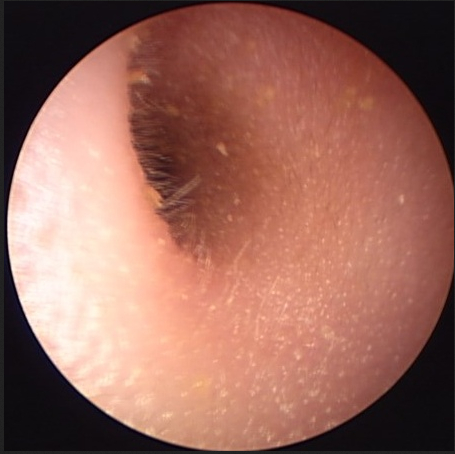
\includegraphics[width=2.5cm]{Figures/Intro/ear1.png}
        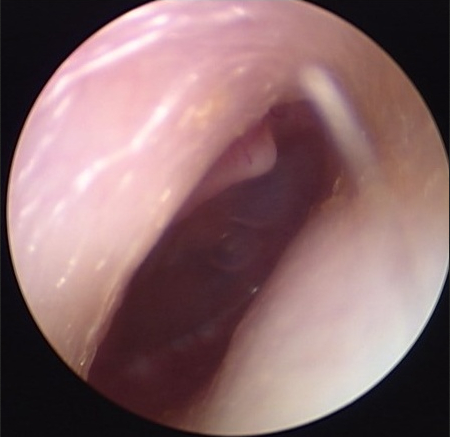
\includegraphics[width=2.5cm]{Figures/Intro/ear2.png}
        \caption{The membrane is not visible}
        \label{fig:intro_not_visible}
    \end{subfigure}
    \caption{Three primary challenges of filtering away otoscopy images of poor quality.}
    \label{fig:intro}
\end{figure}

In this project, the aim is to construct an interactive program to help a doctor take good otoscopy images of the ear drum. A data set of 153 images is used to determine the be best possible methods for detecting the three challenges in figure \ref{fig:intro}.\\
The first challenge to be examined is detecting if the image is blurred \ref{fig:intro_blur}. Detection of blur is one of the most challenging problems to solve in the field of image processing\cite{FM}. A selection of some promising algorithms from \cite{FM} and \cite{JNB} will be tested and evaluated to integrate the best performing one in the final program.\\
Next, different methods for determining if there is too much earwax \ref{fig:intro_wax} will be examined after which the last problem \ref{fig:intro_not_visible} will be examined.\\
After this, an evaluation of the design, implementation and performance of the final program will be reviewed.
